% Theory
\chapter{Θεωρητικό Υπόβαθρο}
\label{chapter:theory}
Στο παρόν κεφάλαιο γίνεται αναφορά στις βασικές αρχές των νευρωνικών δικτύων και τη χρησιμότητά τους στην επεξεργασία και κατανόηση της φυσικής γλώσσας. Πιο συγκεκριμένα, μελετούνται διάφορες αρχιτεκτονικές που χρησιμοποιούνταν ως τώρα, αλλά γίνεται αναφορά και στα σύγχρονα (\emph{state-of-the-art}) μοντέλα.
% Στο παρόν κεφάλαιο γίνεται αναφορά στη βασικές αρχές των νευρωνικών δικτύων, του \emph{IR},  και πιο συγκεκριμένα στα σύγχρονα μοντέλα που χρησιμοποιούνται για την επεξεργασία και κατανόηση της φυσικής γλώσσας.

\section{Τεχνητά Νευρωνικά Δίκτυα}
Τα τεχνητά νευρωνικά δίκτυα (\emph{Artificial Neural Networks - ANN}) αποτελούν υπολογιστικά συστήματα τα οποία είναι εμπνευσμένα από τα βιολογικά νευρωνικά δίκτυα που συναντώνται στη φύση (π.χ στον ανθρώπινο εγκέφαλο). Τα \emph{ANN} αποτελούνται από κόμβους, σε αντιστοιχία με τους νευρώνες, που μπορούν να είναι συνδεδεμένοι με άλλους κόμβους, σε αντιστοιχία με τις συνάψεις του εγκεφάλου.

Η πιο απλή δομή ενός νευρωνικού δικτύου είναι ο νευρώνας (\emph{perceptron}) και μπορεί να παρουσιαστεί με το \autoref{fig:perceptron}. Οι είσοδοι στο νευρώνα πολλαπλασιάζονται με ένα βάρος η κάθε μία και στη συνέχεια αθροίζονται, παράγοντας έτσι το ζυγισμένο άθροισμα των εισόδων. Το αποτέλεσμα του νευρώνα υπολογίζεται με το πέρασμα του αθροίσματος από μία συνάρτηση ενεργοποίησης. Στην απλούστερη περίπτωση η συνάρτηση ενεργοποίησης μπορεί να παραληφθεί και το αποτέλεσμα του αθροίσματος να είναι η έξοδος του συστήματος. Σε περίπτωση που υπάρχει, είναι αυτή που καθορίζει την έξοδο του νευρώνα (αν θα ενεργοποιηθεί ο νευρώνας ή όχι). Υπάρχουν διάφοροι τύποι συναρτήσεων ενεργοποίησης που χρησιμοποιούνται για τεχνητά νευρωνικά δίκτυα με τις κυριότερες\footnote{\url{https://en.wikipedia.org/wiki/Activation_function}}:

\begin{itemize}
    \item \textbf{δυαδική (\emph{binary})} - η έξοδος είναι \{0, 1\}
    \item \textbf{σιγμοειδής (\emph{sigmoid})} - η έξοδος είναι στο [0 1]
    \item \textbf{υπερβολική εφαπτομένη (\emph{tanh})} - η έξοδος είναι στο [-1 1]
    \item \textbf{Rectified Linear Unit - ReLU} -  η οποία θέτει την έξοδο ίση με το μηδέν σε περίπτωση αρνητικών τιμών, διαφορετικά δεν επιδρά στην είσοδο
\end{itemize}

\begin{figure}[!ht]
  \centering
  \captionsetup{justification=centering}
  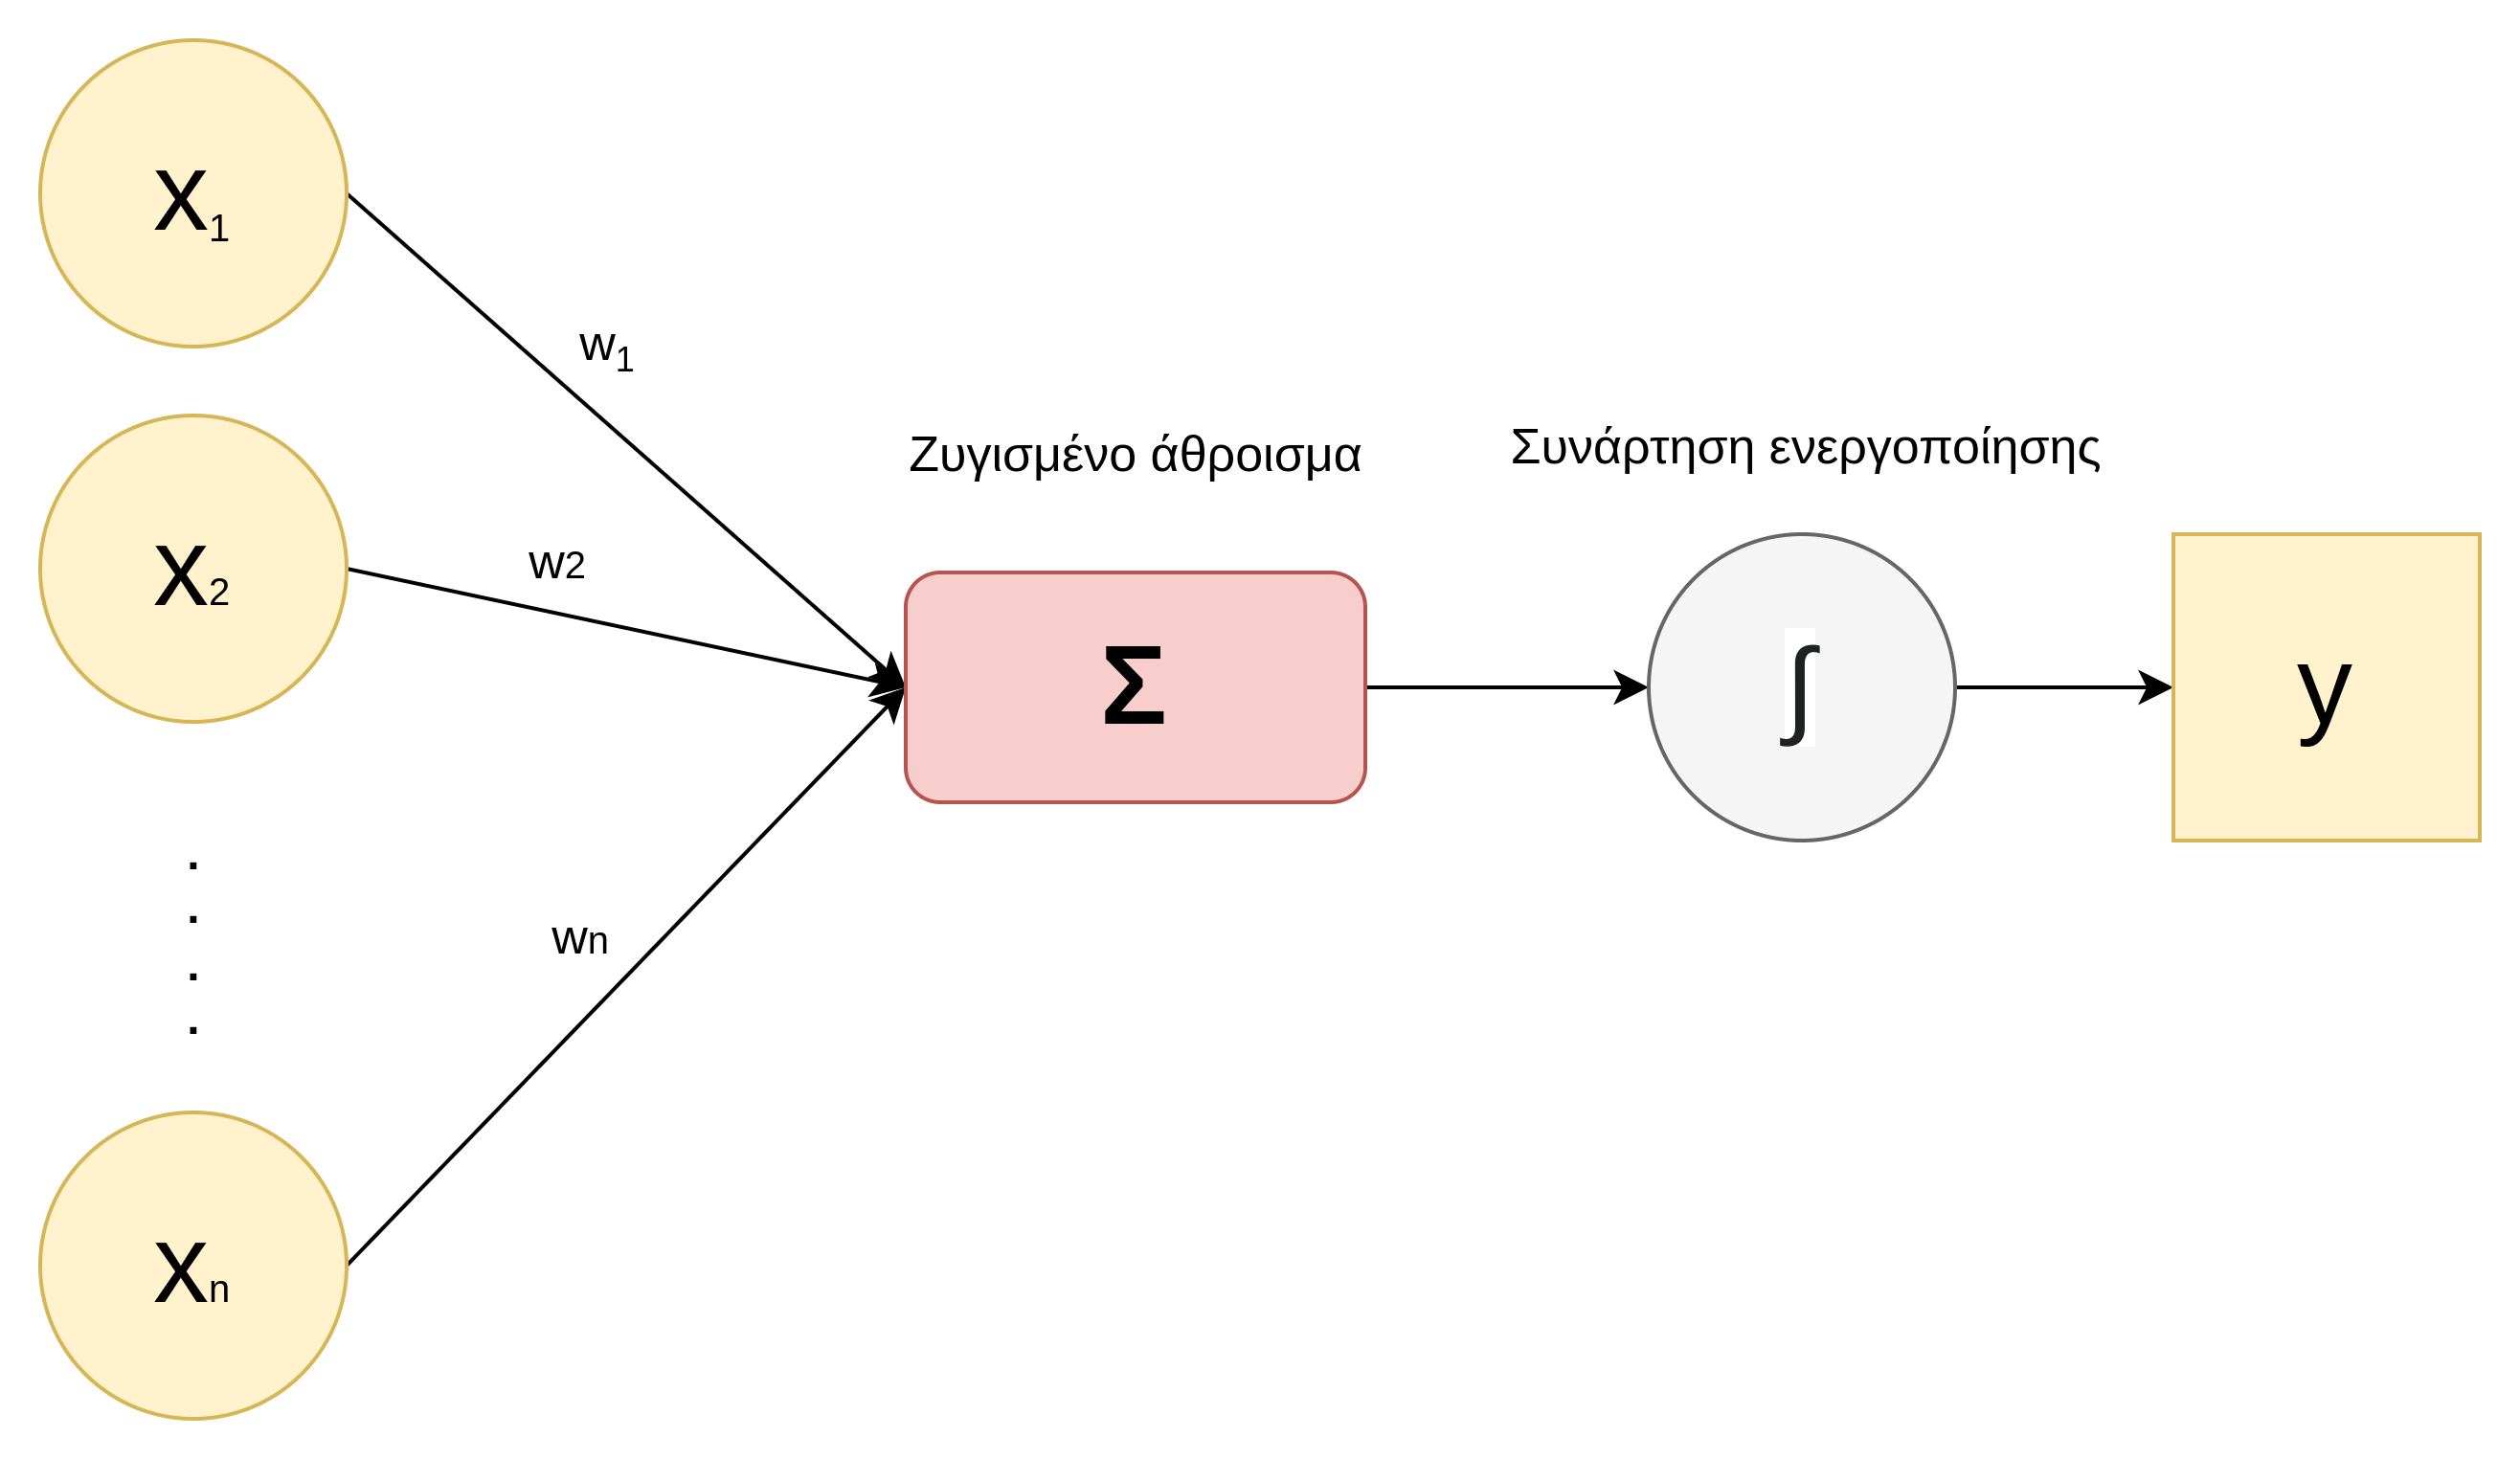
\includegraphics[width=0.7\textwidth]{images/chapter2/perceptron.png}
  \caption{\emph{Νευρώνας - Perceptron}}
  \label{fig:perceptron}
\end{figure}
\noindent

Η σύνδεση πολλών νευρώνων μεταξύ τους δημιουργεί ένα νευρωνικό δίκτυο. Νευρώνες με κοινές εισόδους σχηματίζουν μία ομάδα που ονομάζεται επίπεδο (\emph{layer}). Ένα \emph{NN} μπορεί να αποτελείται από πολλά \emph{layers}. Κάθε επίπεδο που βρίσκεται ανάμεσα στα επίπεδα εισόδου και εξόδου ονομάζεται κρυφό (\emph{hidden layer}). 
Τα \emph{NN} μπορούν να χωριστούν σε δύο κατηγορίες ανάλογα με τη ροή πληροφορίας τους:
\begin{itemize}
    \item \textbf{προς τα εμπρός (\emph{feed forward NN})} - δεν σχηματίζονται κύκλοι ανάμεσα στους κόμβους
    \item \textbf{αναδρομικά (\emph{recurrent NN})} - σχηματίζονται κύκλοι ανάμεσα στους κόμβους
\end{itemize}

Η βασική δομή ενός \emph{NN} φαίνεται στο \autoref{fig:mlp}. Αν κάθε κόμβος από κάθε επίπεδο συνδέεται με κάθε κόμβο του επόμενου επιπέδου τότε το νευρωνικό δίκτυο ονομάζεται πλήρως συνδεδεμένο (\emph{fully connected}). Επίσης, ένα \emph{feed forward NN} ονομάζεται και \emph{Multi-Layer Perceptron - MLP}.

\begin{figure}[!ht]
  \centering
  \captionsetup{justification=centering}
  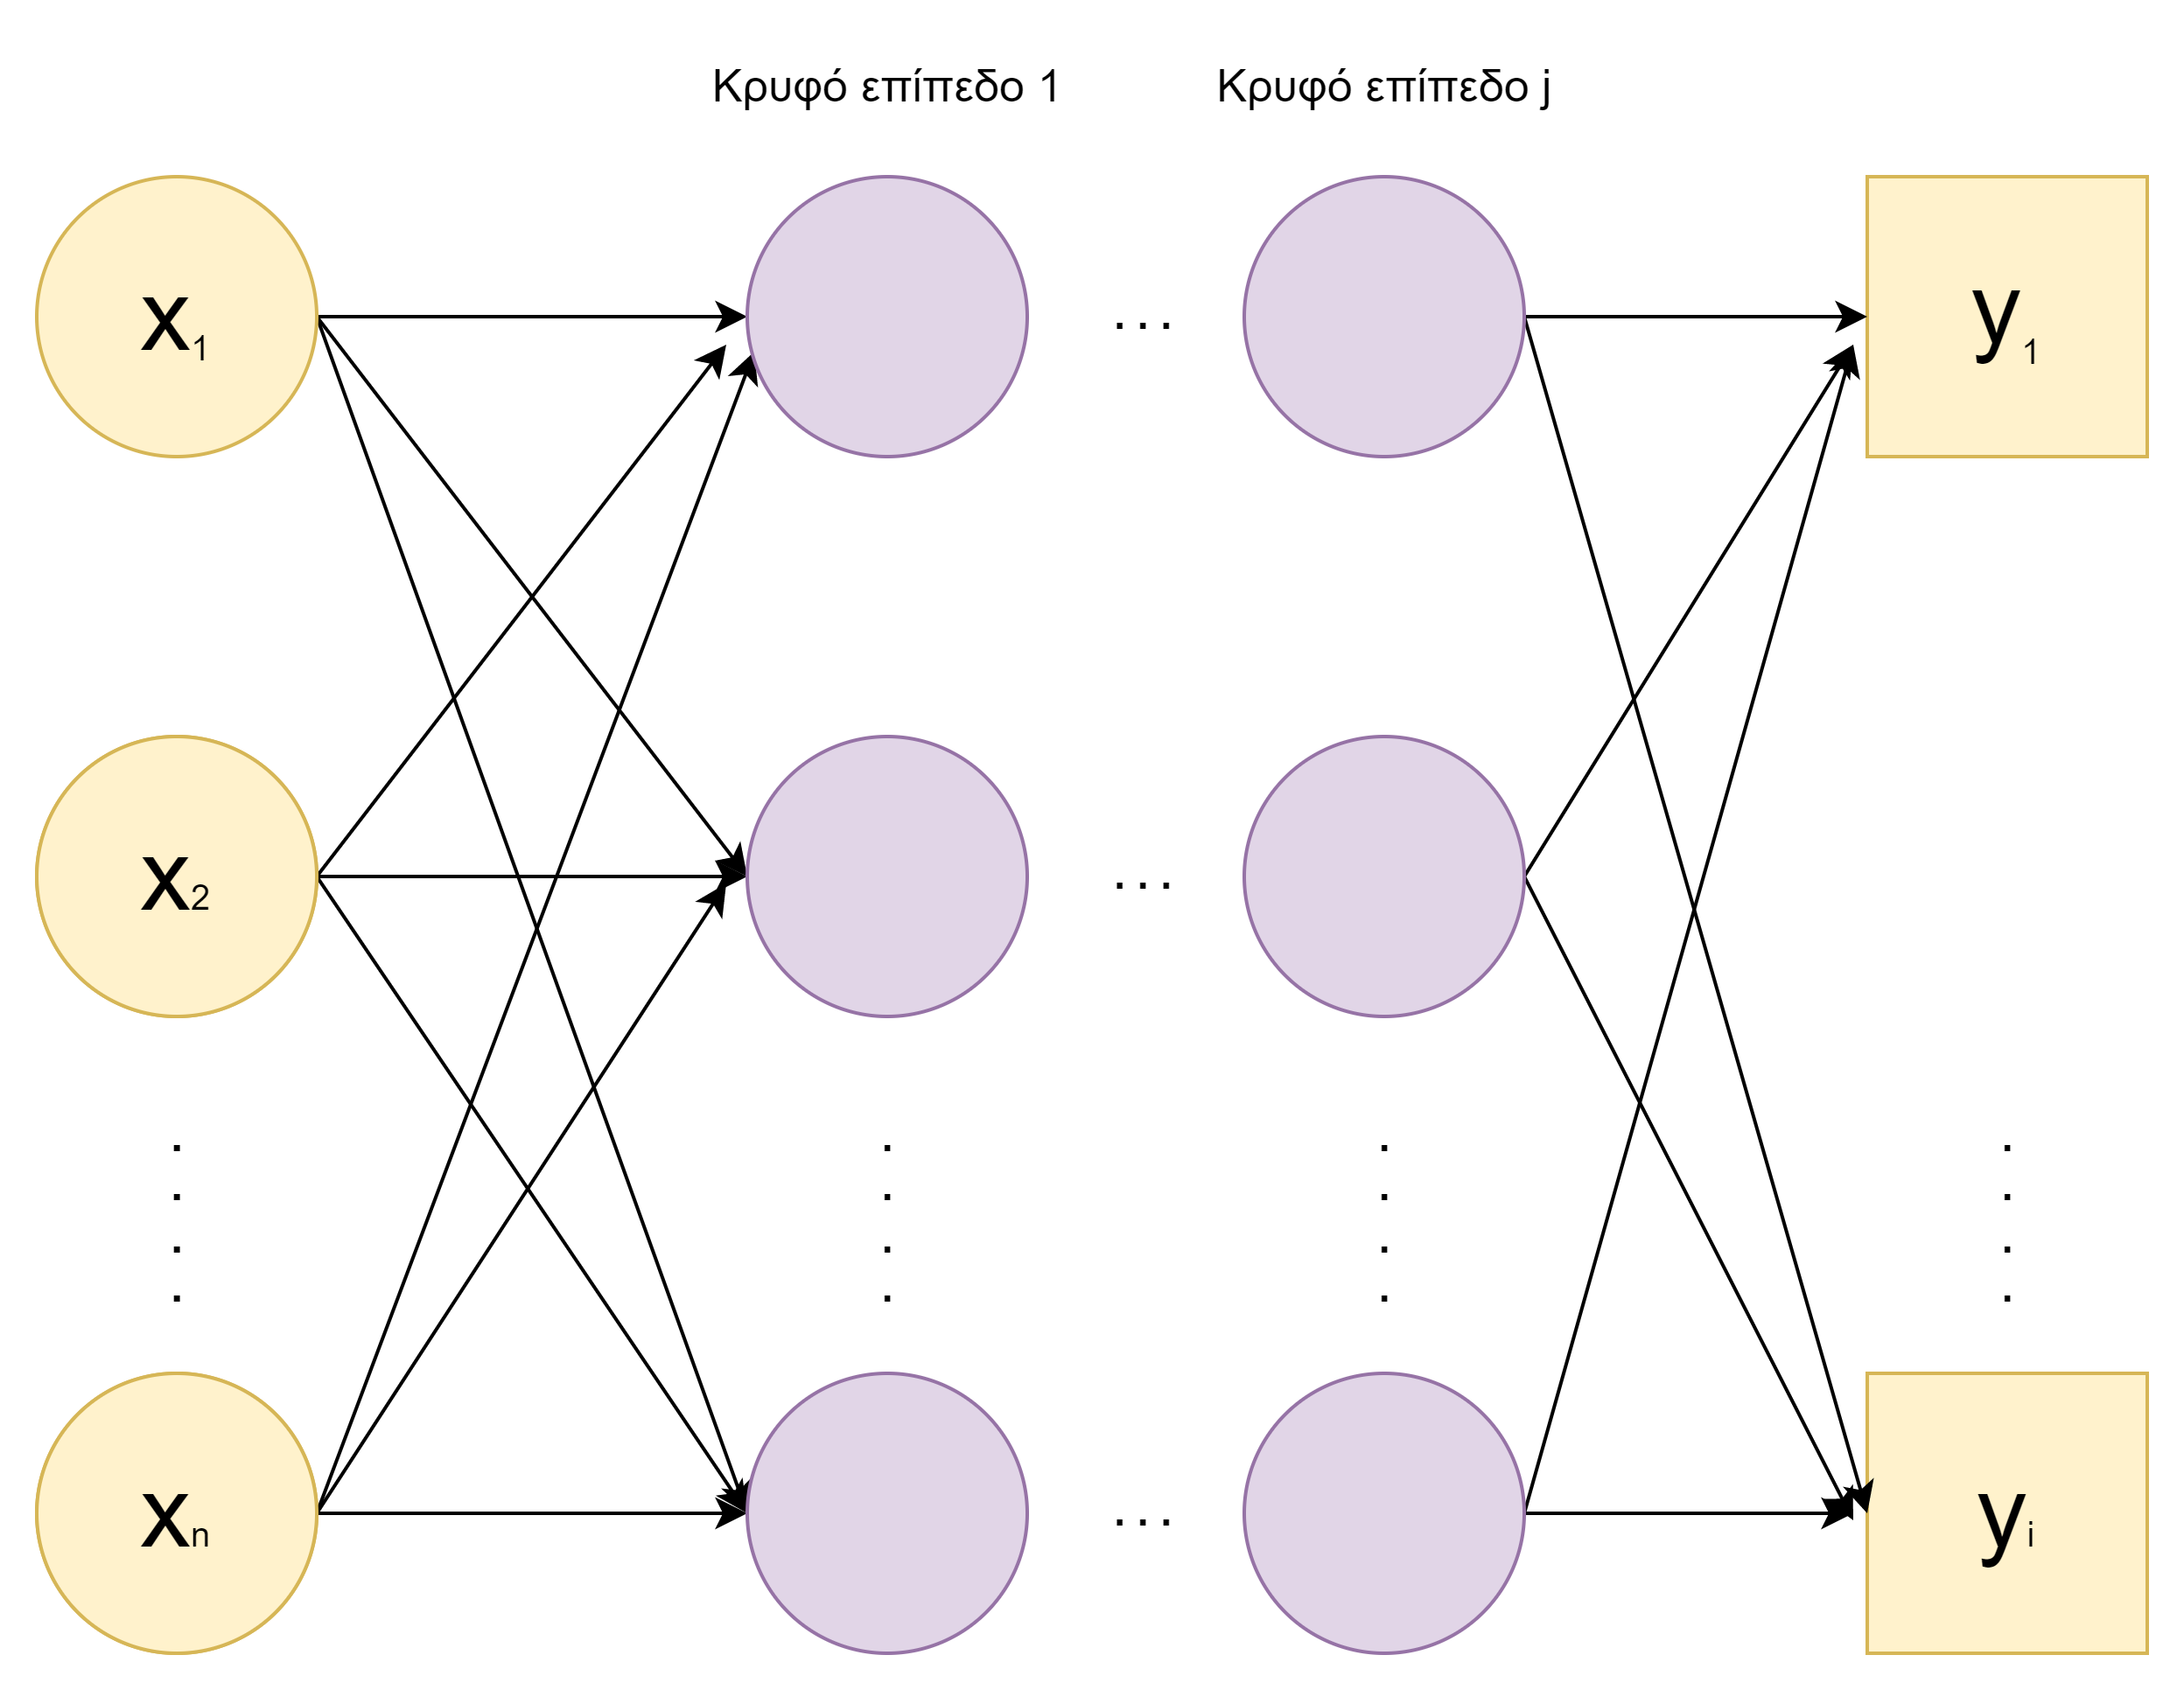
\includegraphics[width=0.7\textwidth]{images/chapter2/mlp.png}
  \caption{\emph{Feed forward Neural Network / Multi Layer Perceptron}}
  \label{fig:mlp}
\end{figure}
\noindent

\section{Ταξινόμηση με \emph{MLP}}
Συχνά μοντέλα \emph{MLP} χρησιμοποιούνται για ταξινόμηση της εισόδου σε κάποια κατηγορία (κλάση). Αν οι διαθέσιμες κλάσεις ταξινόμησης είναι δύο, τότε η έξοδος του \emph{NN} είναι μία και μπορεί να παίρνει τις τιμές $0$ ή $1$, επομένως στο τέλος χρησιμοποιείται μία \emph{sigmoid} συνάρτηση ενεργοποίησης. Σε περίπτωση που οι κλάσεις είναι περισσότερες, τότε οι έξοδοι του έχει νόημα να εκφράζουν μία συνάρτηση μάζας πιθανότητας. Πιο συγκεκριμένα, κάθε μία από τις εξόδους εκφράζει την πιθανότητα η είσοδος να ανήκει σε μία από τις κλάσεις. Το συνολικό άθροισμα των πιθανοτήτων αυτών είναι μονάδα. Η έξοδος με τη μεγαλύτερη πιθανότητα καθορίζει και την κλάση ταξινόμησης της εισόδου. Αυτό επιτυγχάνεται με τη συνάρτηση \emph{softmax} η οποία φαίνεται στην \autoref{eq:softmax}.

\begin{equation}
    \label{eq:softmax}
    \text{y}(x_{i}) = \text{softmax}(x_{i}) = \frac{\exp(x_i)}{\sum_1^j \exp(x_j)}
\end{equation}

\section{Αναδρομικά Νευρωνικά Δίκτυα}
Τα απλά \emph{feed forward} νευρωνικά δίκτυα παράγουν την έξοδο τους βασιζόμενα μόνο στα δεδομένα της τρέχουσας εισόδου. Ωστόσο, πολλές φορές η πληροφορία που παρέχεται από τα προηγούμενα δείγματα της εισόδου ενδέχεται να επηρεάζει το αποτέλεσμα της επόμενης εξόδου. Το πρόβλημα αυτό έρχονται να λύσουν τα Αναδρομικά Νευρωνικά Δίκτυα (\emph{Recurrent Neural Networks - RNN}). Ένα \emph{RNN}, \autoref{fig:rnn}, μπορεί να θεωρηθεί ως πολλά αντίγραφα ενός απλού νευρωνικού δικτύου με το κάθε ένα να παρέχει την έξοδο του στο επόμενο. Η έξοδος αυτή ονομάζεται κρυφή κατάσταση (\emph{hidden state}) και είναι αυτή που παρέχει τη "μνήμη" στο συνολικό σύστημα. Αυτή η αλυσιδωτή δομή επιτρέπει την πρόβλεψη σειριακών δεδομένων όπως χρονοσειρές, ήχο, βίντεο, δεδομένα καιρού, κείμενο και άλλων.

\begin{figure}[!ht]
  \centering
  \captionsetup{justification=centering}
  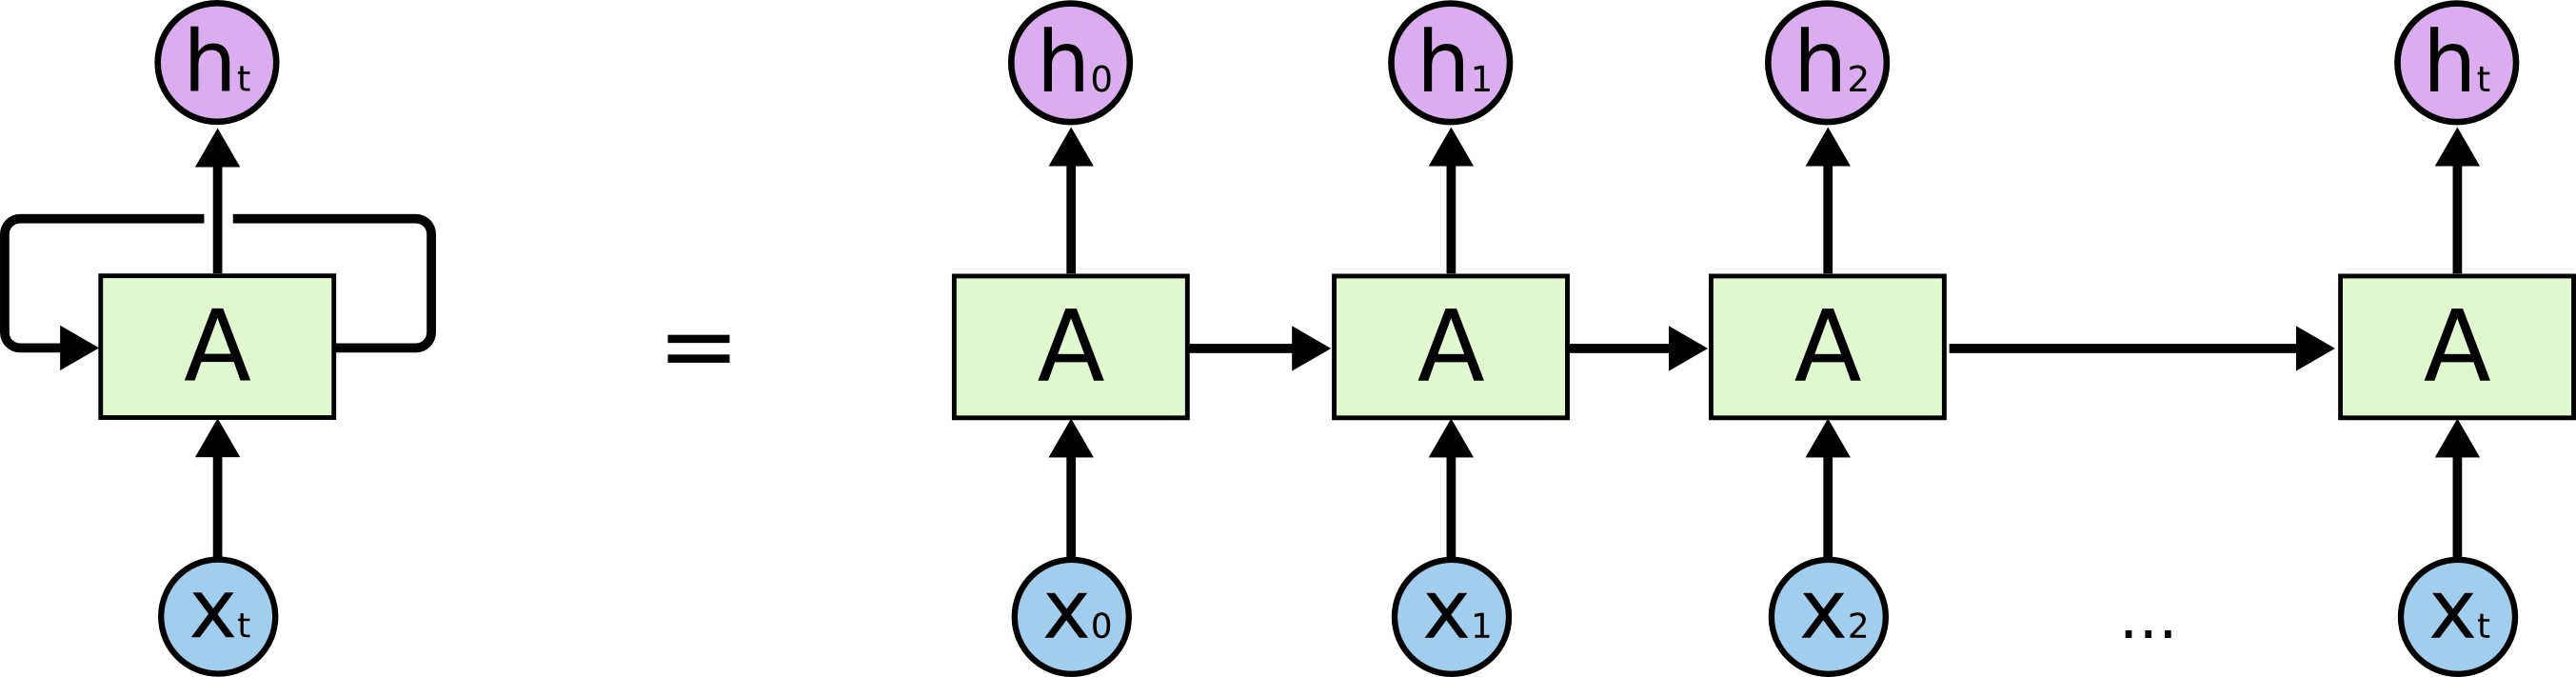
\includegraphics[width=0.7\textwidth]{images/chapter2/rnn.png}
  \captionsource{\emph{Recurrent Neural Network}}{\url{https://colah.github.io/posts/2015-08-Understanding-LSTMs}}
  \label{fig:rnn}
\end{figure}
\noindent

\subsection{Νευρωνικά Δίκτυα Μακροπρόθεσμης Μνήμης}
Παρά το γεγονός ότι τα \emph{RNN} στη θεωρία μπορούν να διαχειρίζονται συνδέσεις των δεδομένων διάφορων εισόδων, όσο εισέρχονται νέα δείγματα στο σύστημα τόσο δυσκολότερη είναι η σύνδεση με τα πιο παλιά. Αυτό το πρόβλημα είναι γνωστό στη βιβλιογραφία ως \emph{vanishing gradient descent}. Μία νέα αρχιτεκτονική, τα μοντέλα μακροπρόθεσμης μνήμης (\emph{Long-Short Term Memory - LSTM}), η οποία παρουσιάζεται στο \autoref{fig:lstm-arch}, λύνει το συγκεκριμένο πρόβλημα. Το βασικότερο στοιχείο ενός \emph{LSTM} είναι η κατάσταση του (\emph{cell state - C}), στο οποίο διατηρείται η πληροφορία από τα προηγούμενα επίπεδα. Σε κάθε επόμενο επίπεδο παρέχεται η πληροφορία του \emph{cell state} του προηγούμενου επιπέδου και υπάρχει η δυνατότητα προσθήκης και αφαίρεσης πληροφορίας σε αυτό.

\begin{figure}[!ht]
  \centering
  \captionsetup{justification=centering}
  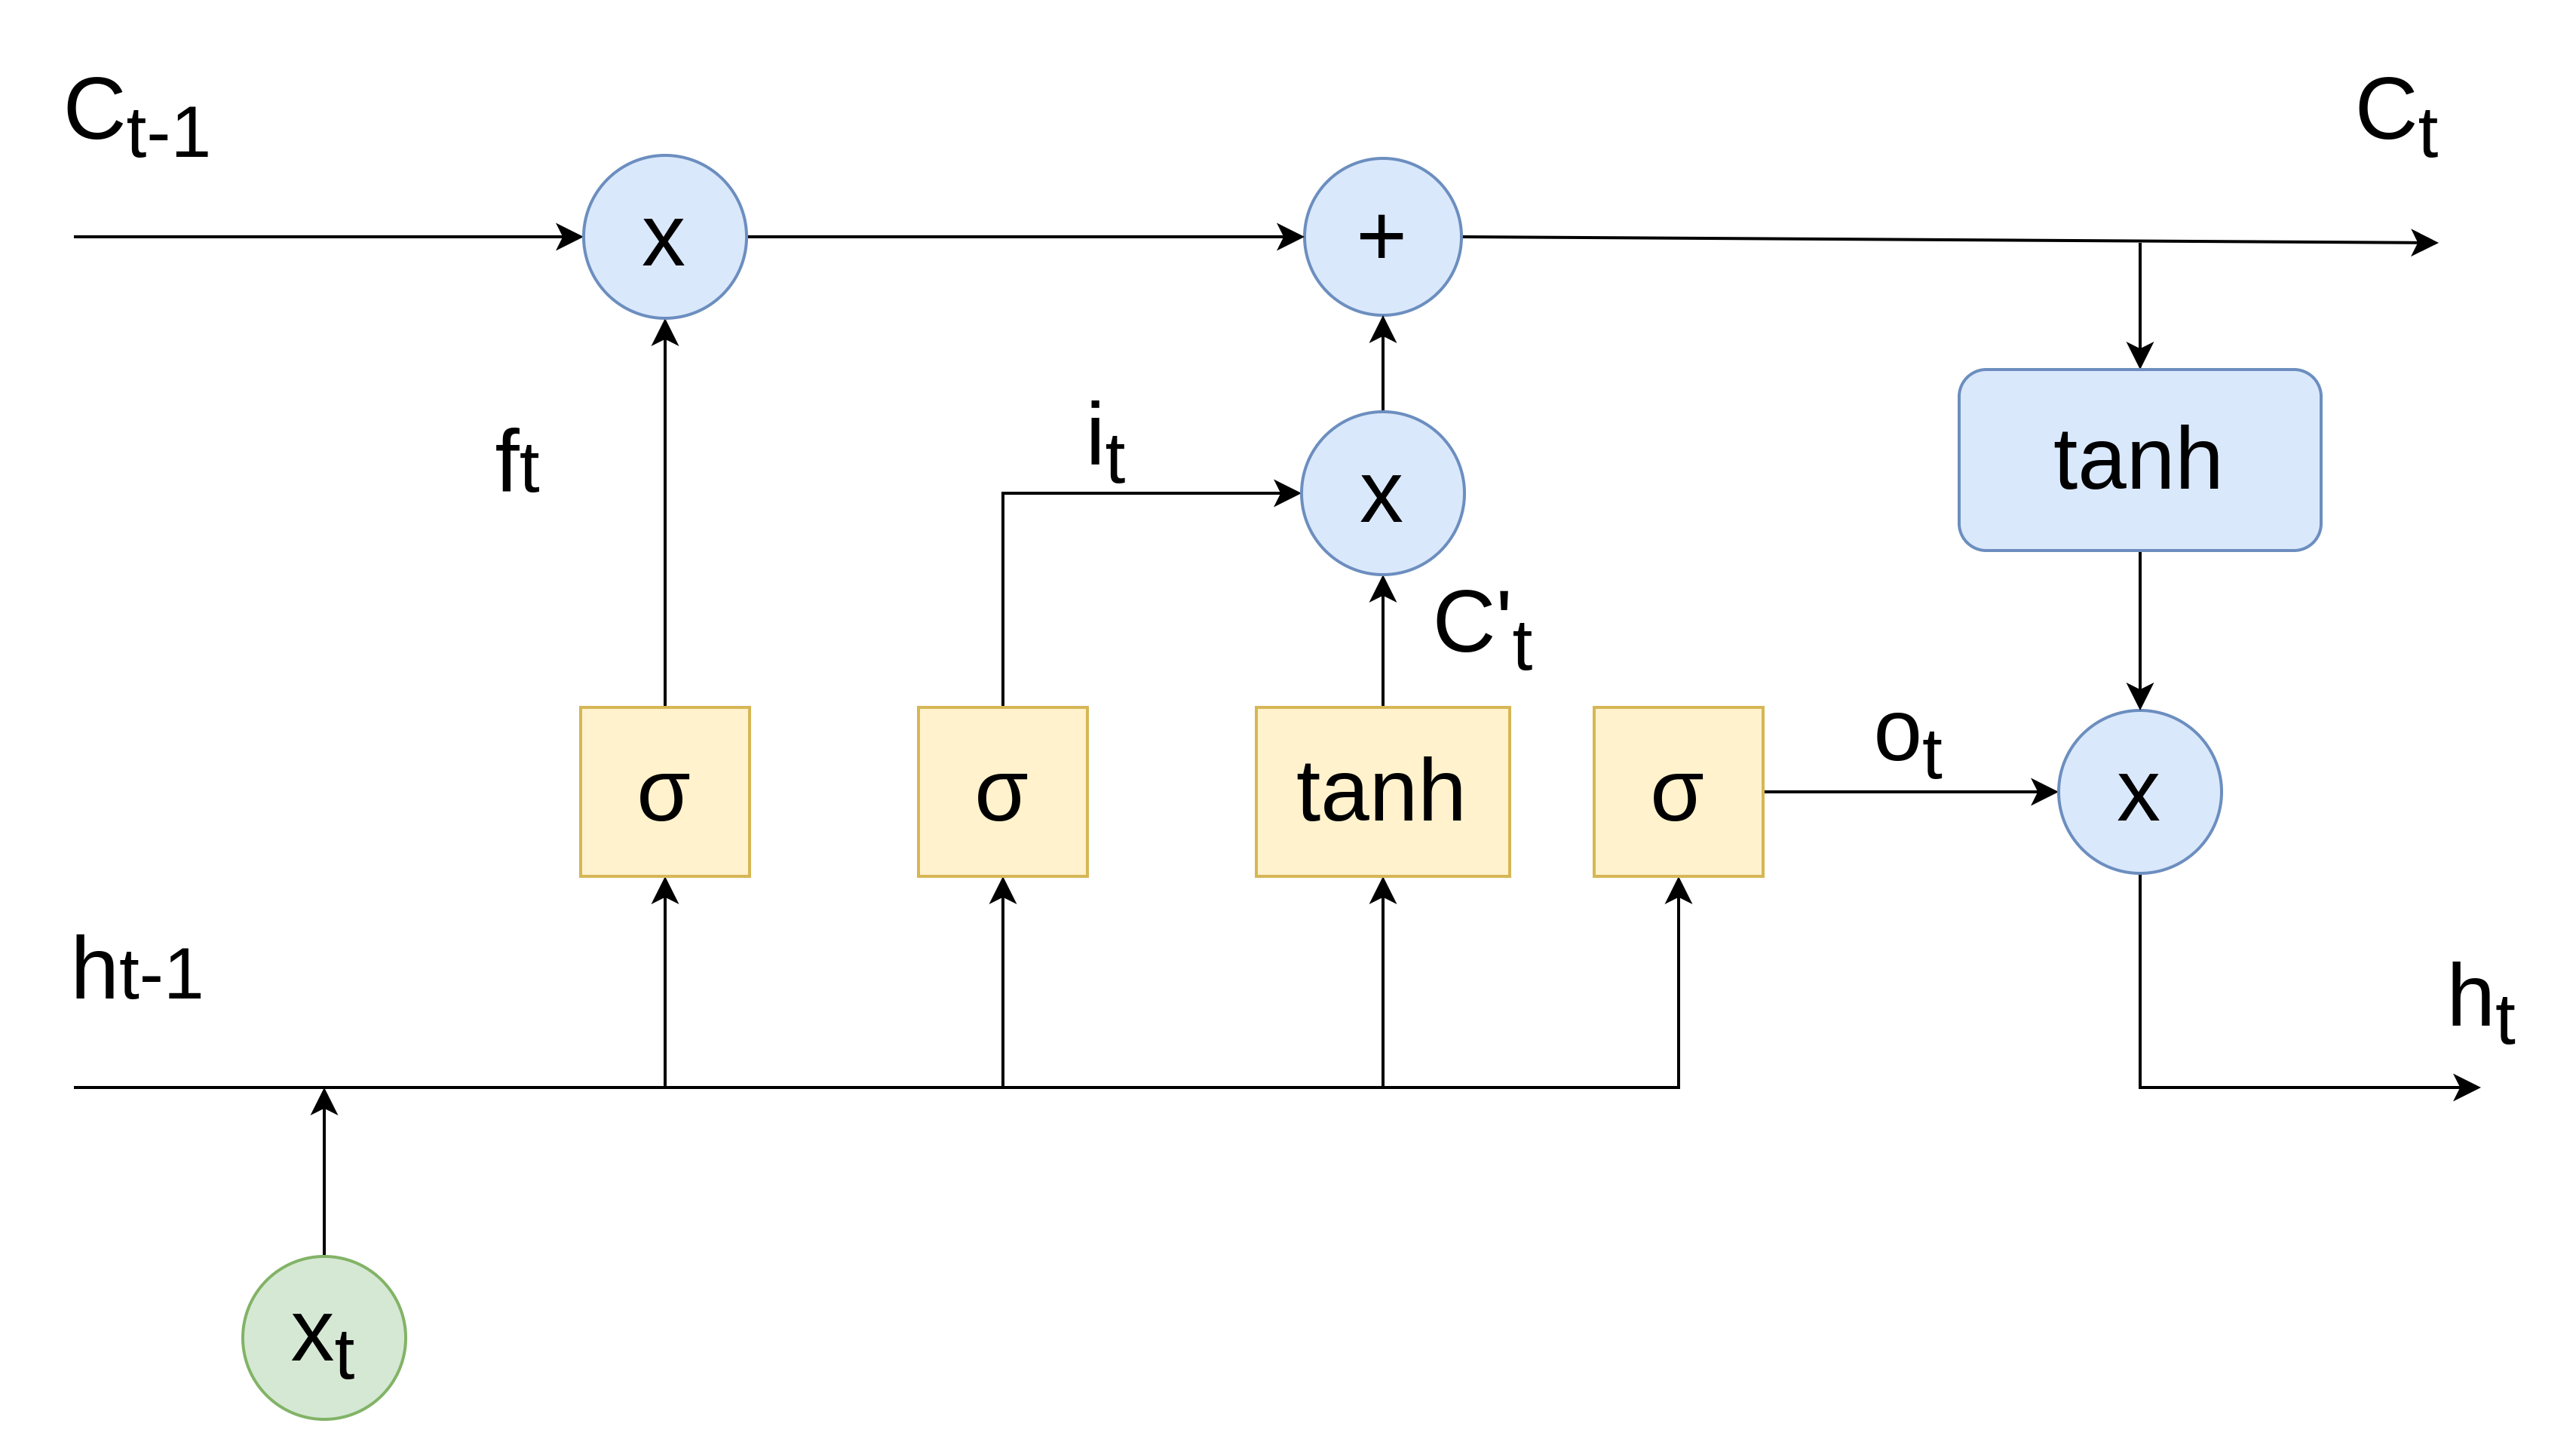
\includegraphics[width=0.7\textwidth]{images/chapter2/lstm-arch.png}
  \captionsource{\emph{Αρχιτεκτονική LSTM}}{\url{https://colah.github.io/posts/2015-08-Understanding-LSTMs}}
  \label{fig:lstm-arch}
\end{figure}
\noindent

Ο τρόπος με τον οποίο γίνεται η ανανέωση της πληροφορίας περιγράφεται στη συνέχεια. Κάθε ένα από τα στάδια επεξεργασίας μπορεί να παρομοιαστεί με το πέρασμα από μία πύλη. Στο πρώτο βήμα, πραγματοποιείται η απόφαση για το ποια πληροφορία από το προηγούμενο \emph{cell state} θα παραληφθεί, πύλη \emph{forget}. Πιο συγκεκριμένα, χρησιμοποιεί πληροφορία από το προηγούμενο επίπεδο σε συνδυασμό με την είσοδο. Η πληροφορία περνάει από μία σιγμοειδή συνάρτηση ενεργοποίησης που έχει ως έξοδο ένα διάνυσμα αριθμών, με τόσες θέσεις όσες και το $C_{t-1}$, στο διάστημα [0 1] όπου το 0 μεταφράζεται σε απόρριψη του συγκεκριμένου κελιού και το ένα σε διατήρηση του. Στη συνέχεια, γίνεται ο υπολογισμός δύο διανυσμάτων, ενός για ανανέωση ήδη υπάρχουσας πληροφορίας ($i_t$ ,χρησιμοποιώντας ξανά σιγμοειδή συνάρτηση ενεργοποίησης) και ενός για προσθήκη νέας ($C_t'$, χρησιμοποιώντας \emph{tanh} συνάρτηση ενεργοποίησης), πύλη ανανέωσης/προσθήκης. Από τον συνδυασμό των δύο διανυσμάτων αυτών προκύπτει η νέα κατάσταση \emph{C}. Η συνολική κατάσταση του επιπέδου μπορεί να περιγραφεί με τις παρακάτω εξισώσεις\footnote{Το σύμβολο $\circ$ υποδηλώνει πολλαπλασιασμό στοιχείο προς στοιχείο}:
\begin{itemize}
    \item $f_t$ = $\sigma(W_f x_t + U_f h_{t-1} + b_f)$
    \item $i_t$ = $\sigma(W_i x_t + U_i h_{t-1} + b_i)$
    \item $o_t$ = $\sigma(W_o x_t + U_o h_{t-1} + b_o)$
    \item $C_t'$ = $\sigma(W_c x_t + U_c h_{t-1} + b_c)$
    \item $C_t$ = $f_t \circ c_{t-1} + i_t \circ C_t'$
    \item $h_t$ = $o_t \circ \sigma(C_t)$
\end{itemize}

όπου: 
\begin{itemize}
    \item $x_t$: είσοδος του \emph{LSTM}
    \item $f_t$: διάνυσμα που προκύπτει από την πύλη \emph{forget}
    \item $i_t$: διάνυσμα που προκύπτει από την πύλη ανανέωσης/προσθήκης
    \item $o_t$: διάνυσμα που προκύπτει από την πύλη εξόδου
    \item $h_t$: διάνυσμα κρυφής κατάστασης του \emph{LSTM}
    \item $C_t'$: διάνυσμα για τη προσθήκη νέας πληροφορίας
    \item $C_t$: διάνυσμα κατάστασης του \emph{LSTM}
    \item W, U: πίνακες με τα βάρη που προκύπτουν από την εκπαίδευση του μοντέλου
    \item $b_f$ : είναι ένα \emph{bias} διάνυσμα που προκύπτει από την εκπαίδευση του μοντέλου
\end{itemize}

\section{Αναπαράσταση Λέξεων σε Διανύσματα}
Για να γίνει δυνατή η επεξεργασία της φυσικής γλώσσας από νευρωνικά δίκτυα πρέπει πρώτα κάθε λέξη να αποκτήσει μορφή η οποία μπορεί να επεξεργαστεί από αυτά. Οι λέξεις μετατρέπονται σε διανύσματα, τα οποία ονομάζονται \emph{word embeddings}.

\subsection{Δημιουργία Λεξιλογίου/Συμβολισμού}
Η δημιουργία λεξιλογίου, \emph{tokenization}, είναι μία διαδικασία διαχωρισμού κειμένου σε μικρότερα κομμάτια που ονομάζονται σύμβολα (\emph{tokens}). Τα σύμβολα του λεξιλογίου μπορεί να είναι ή ολόκληρες λέξεις (\emph{word tokenization}) ή χαρακτήρες (\emph{character tokenization}) ή υπό-λέξεις (\emph{n-gram tokenization}, όπου n ο αριθμός των \emph{tokens} που μπορούν να συνδυαστούν για την παραγωγή μιας λέξης). Συνήθως τα μοντέλα επεξεργασίας φυσικής γλώσσας χρησιμοποιούν λεξιλόγια που χρησιμοποιούν συνδυασμό των παραπάνω τεχνικών για την κάλυψη μεγάλου εύρους της φυσικής γλώσσας. Μέσω του λεξιλογίου μπορεί να παραχθεί, όπως παρουσιάζεται στη συνέχεια, μία αντιστοίχηση της φυσικής γλώσσας σε αριθμητικά διανύσματα τα οποία μπορούν στη συνέχεια να επεξεργαστούν από νευρωνικά δίκτυα. 

\subsection{One-hot Encoding}
Η \emph{one-hot encoding} αποτελεί από τις πιο απλές αναπαραστάσεις προτάσεων σε διάνυσμα. Κάθε πρόταση αναπαρίσταται από ένα διάνυσμα με διάσταση όσο και το μέγεθος του λεξιλογίου. Το λεξιλόγιο είναι το σύνολο με κάθε πιθανή λέξη  που μπορεί να εμφανιστεί σε μία πρόταση. Κάθε θέση στο διάνυσμα αντιστοιχεί σε μία λέξη του λεξιλογίου. Έτσι αν μία λέξη εμφανίζεται στη πρόταση εισόδου τότε η αντίστοιχη τιμή στο διάνυσμα τίθεται $1$ διαφορετικά $0$, \autoref{fig:vector}.

\subsection{Bag of Words/Count Encoding}
Η τεχνική \emph{bag of words} ακολουθεί την ίδια διαδικασία δημιουργίας του διανύσματος με τη διαφορά ότι κάθε κελί του διανύσματος δείχνει τη συχνότητα εμφάνισης της αντίστοιχης λέξης του λεξιλογίου, \autoref{fig:vector}.

\begin{figure}[!ht]
  \centering
  \captionsetup{justification=centering}
  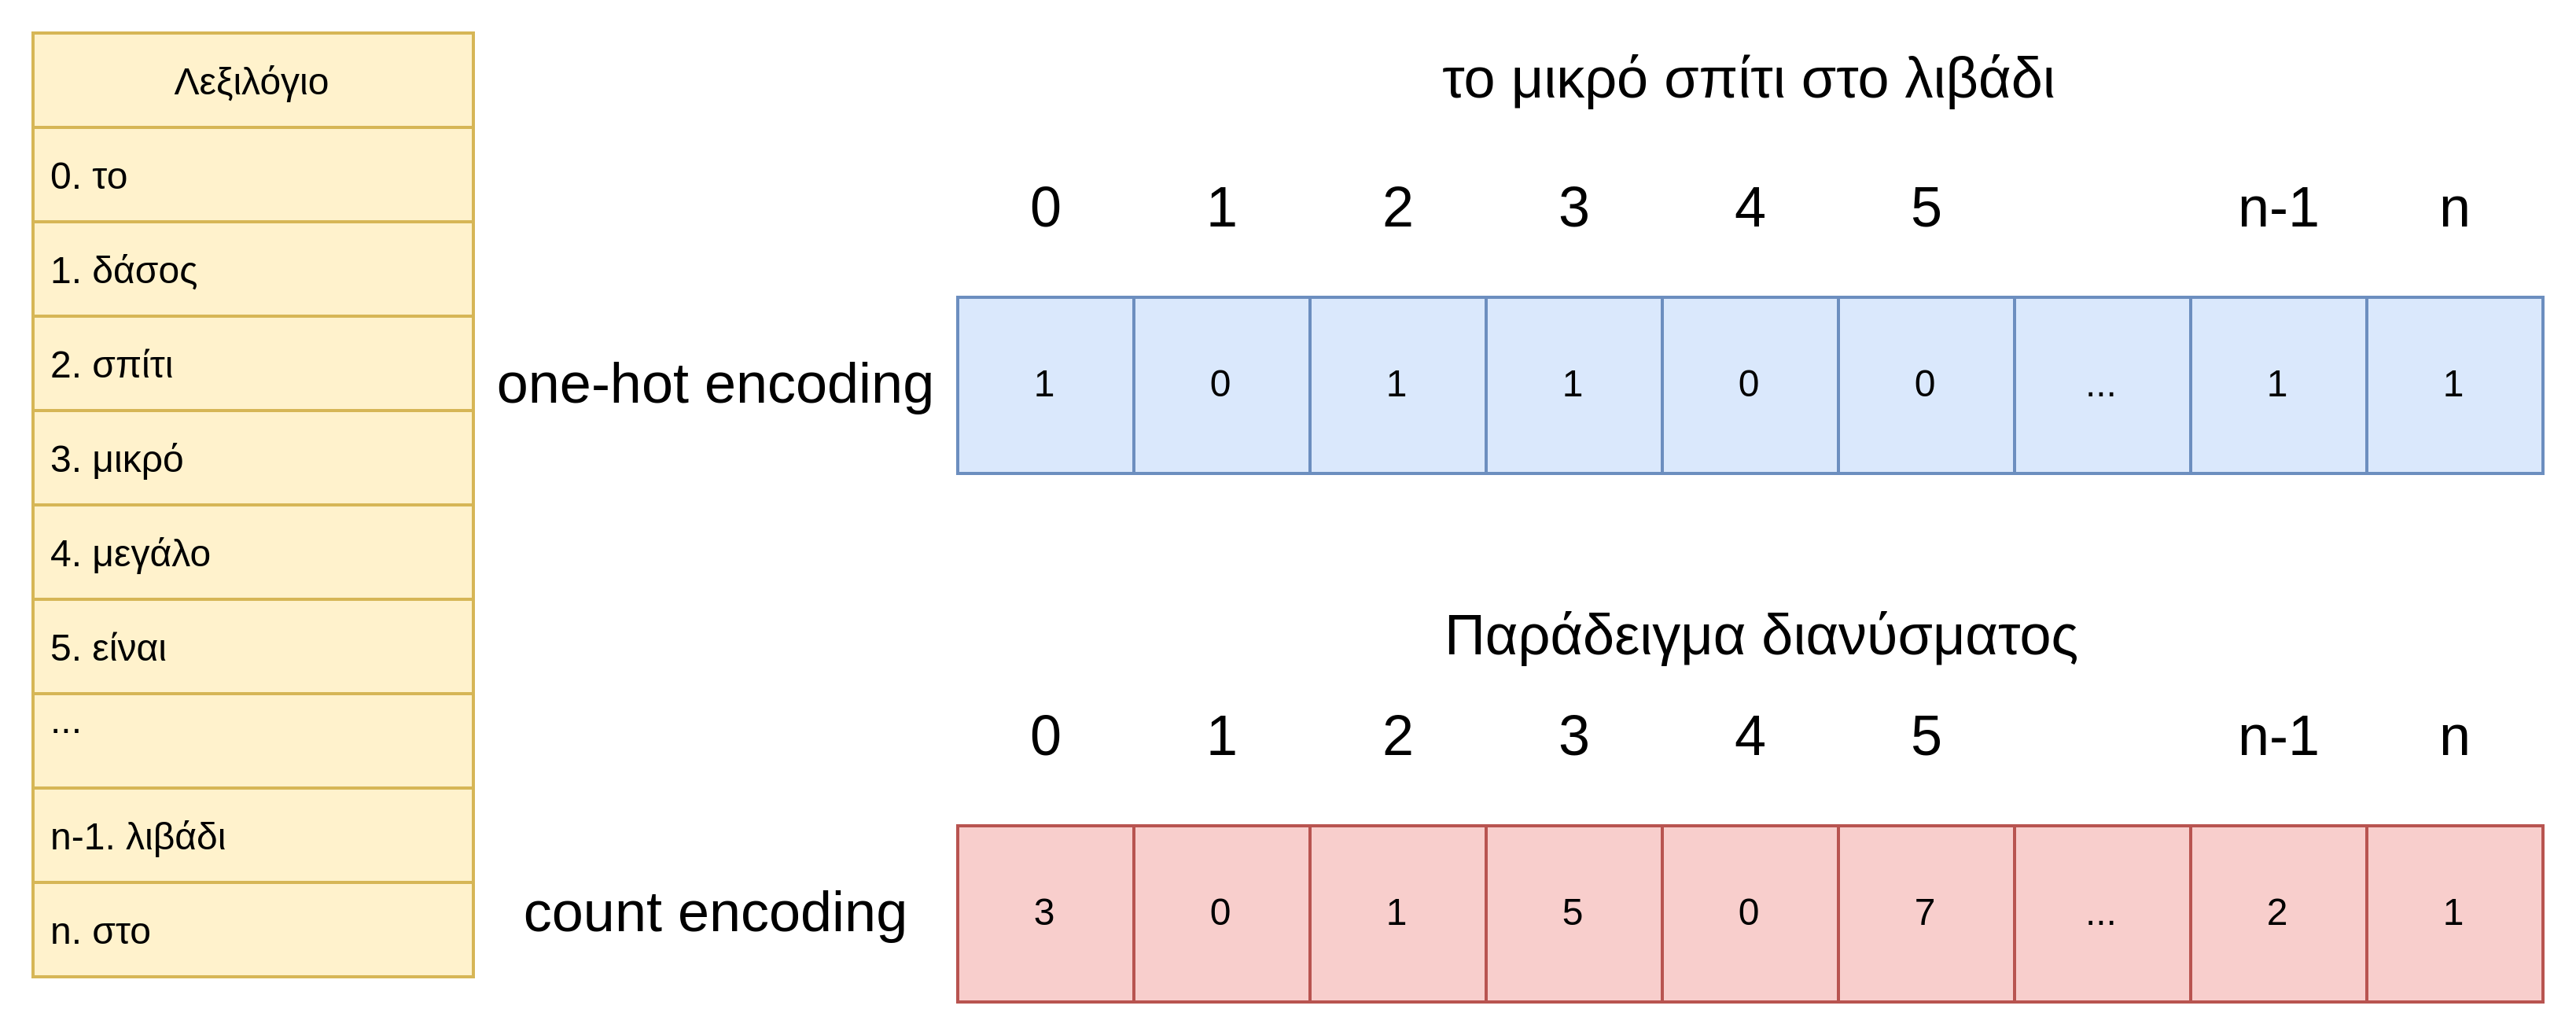
\includegraphics[width=0.7\textwidth]{images/chapter2/vector.png}
  \caption{Παράδειγμα διανυσμάτων \emph{one-hot encoding \& count encoding}}
  \label{fig:vector}
\end{figure}
\noindent

\subsection{Συχνότητα Εμφάνισης Όρου - Αντίστροφη Συχνότητα Εμφάνισης Εγγράφου}
Μία από τις πιο δημοφιλής τεχνικές δημιουργίας \emph{word embeddings} είναι η Συχνότητα Εμφάνισης Όρου - Αντίστροφη συχνότητα Εμφάνισης Εγγράφου (\emph{Term Frequency - Inverse Document Frequency - TF-IDF}). Αποτελεί μία στατιστική μέθοδο η οποία δείχνει πόσο σημαντική είναι μία λέξη σε ένα σύνολο από έγγραφα. Ο υπολογισμός της προκύπτει από το γινόμενο της συχνότητας εμφάνισης (\emph{Term Frequency - TF}) της λέξης στο αντίστοιχο έγγραφο, όπως και στο \emph{bag of words}, επί την αντίστροφη συχνότητα της λέξης σε όλα τα έγγραφα (\emph{Inverse Document Frequency - IDF}). Έστω ένα σύνολο από έγγραφα $D$ και έστω $t$ η λέξη της οποίας αναζητείται η \emph{TF-IDF} τότε:

\begin{equation}
    \label{eq:tfidf}
    \text{TF-IDF}(t,d) = TF \cdot \log {\frac{ |D| }{ 1 + | \{ f \in D : t \in f \} |}}
\end{equation}

όπου, στην \autoref{eq:tfidf}:

\begin{itemize}
    \item \emph{t}: η λέξη
    \item \emph{d}: το έγγραφο
    \item TF: το πλήθος των φορών που εμφανίζεται η λέξη στο αντίστοιχο έγγραφο
    \item |D|: ο συνολικός αριθμός των εγγράφων
    \item $| \{ f \in D : t \in f \} |$: το πλήθος των εγγράφων που εμφανίζεται η λέξη \emph{t}
\end{itemize}

Η μέθοδος \emph{TF-IDF} μπορεί επίσης να χρησιμοποιηθεί και για \emph{IR}. Έστω μια πρόταση της οποίας αναζητείται το πλησιέστερο έγγραφο. Για κάθε έγγραφο υπολογίζεται η μετρική \emph{TF-IDF} ως το άθροισμα των \emph{TF-IDF} κάθε λέξης στην πρόταση. Τα έγγραφα με τις μεγαλύτερες τιμές είναι και τα πιο πιθανά να σχετίζονται με την αρχική πρόταση.

\begin{equation}
    \label{eq:total-tfidf}
    \text{TF-IDF}(Q,d) = \sum_{t \in Q} TF \cdot \log {\frac{ |D| }{ 1 + | \{ f \in D : t \in f \} |}}
\end{equation}
όπου, στην \autoref{eq:total-tfidf}:
\begin{itemize}
    \item Q: η πρόταση
    \item t: μία λέξη της πρότασης
\end{itemize}

Παρά το γεγονός ότι η παραπάνω μέθοδος είναι αρκετά αποδοτική έχει δύο βασικά μειονεκτήματα. Όπως είναι εύκολα παρατηρήσιμο, όσο αυξάνεται η συχνότητα εμφάνισης της λέξης στο έγγραφο τόσο αυξάνεται και το σκορ της, χωρίς ωστόσο αυτό να σημαίνει ότι το συγκεκριμένο έγγραφο είναι πιο σχετικό με την αρχική πρόταση. Επιπλέον, η \emph{TF-IDF} δεν λαμβάνει καθόλου υπόψιν το μέγεθος του εγγράφου.

\subsection{\emph{BM25}}
Το σκορ \emph{BM25} είναι μία παραλλαγή του \emph{TF-IDF} που αναγνωρίζει τις αδυναμίες που αναφέρθηκαν παραπάνω και τις αντιμετωπίζει βασίζόμενο στην επιλογή δύο παραμέτρων. Η παράμετρος $k_1$ είναι υπεύθυνη για τον κορεσμό του \emph{TF} σε περίπτωση που κάποιος όρος εμφανίζεται πολλές φορές στο αντίστοιχο έγγραφο. Πιο συγκεκριμένα, το σκορ αυξάνεται γρήγορα στις αρχικές εμφανίσεις της λέξης στο κείμενο και σταδιακά επηρεάζει λιγότερο την άνοδο του σκορ. Επιπλέον, εισάγει την παράμετρο $b$ η οποία καθορίζει πόσο θα επηρεάζεται το σκορ από το μέγεθος του εγγράφου. Έτσι,προκύπτει η \autoref{eq:bm25}:

\begin{equation}
    \label{eq:bm25}
    \text{BM25}(Q,d) = \sum_{t \in Q} \frac{TF}{TF + k_1 \cdot (1 - b + b \cdot \frac{len_{doc}}{len_{avg}})} \cdot \log {\frac{|D| + 1}{| \{ f \in D : t \in f \} | + 0.5}}
\end{equation}

όπου:
\begin{itemize}
    \item Q: η πρόταση
    \item d: το αρχείο του οποίου το σκορ υπολογίζεται
    \item t: μία λέξη από την πρόταση Q
    \item TF: η συχνότητα εμφάνισης της λέξης στο έγγραφο d
    \item $len_{doc}$: το μέγεθος του εγγράφου d
    \item $len_{avg}$: ο μέσος όρος του μεγέθους όλων των εγγράφων
    \item |D|: ο συνολικός αριθμός των εγγράφων
    \item $| \{ f \in D : t \in f \} |$: το πλήθος των εγγράφων που εμφανίζεται η λέξη \emph{t}
\end{itemize}

\section{Transformer}
Τα αναδρομικά νευρωνικά δίκτυα αλλά και τα \emph{LSTM} μονοπωλούσαν για αρκετά χρόνια την επίλυση προβλημάτων που απαιτούσαν επεξεργασία σειριακής πληροφορίας, όπως αυτά των \emph{NLP} και \emph{NLU}. Τα \emph{Transformer} παρουσιάστηκαν για πρώτη φορά το $2017$ στο άρθρο \emph{"Attention is all you need"} \cite{attention} και έφεραν στο προσκήνιο μία νέα αρχιτεκτονική για την επίλυση τέτοιου είδους προβλημάτων, \autoref{fig:transformer}. Πιο συγκεκριμένα, το \emph{Transformer} αποτελείται από $N$ επίπεδα κωδικοποίησης, $N$ επίπεδα αποκωδικοποίησης και εστιάζει στη μέθοδο της προσοχής (\emph{attention}) για να διακρίνει ποια κομμάτια της εισόδου είναι πιο σημαντικά.

\begin{figure}[!ht]
  \centering
  \captionsetup{justification=centering}
  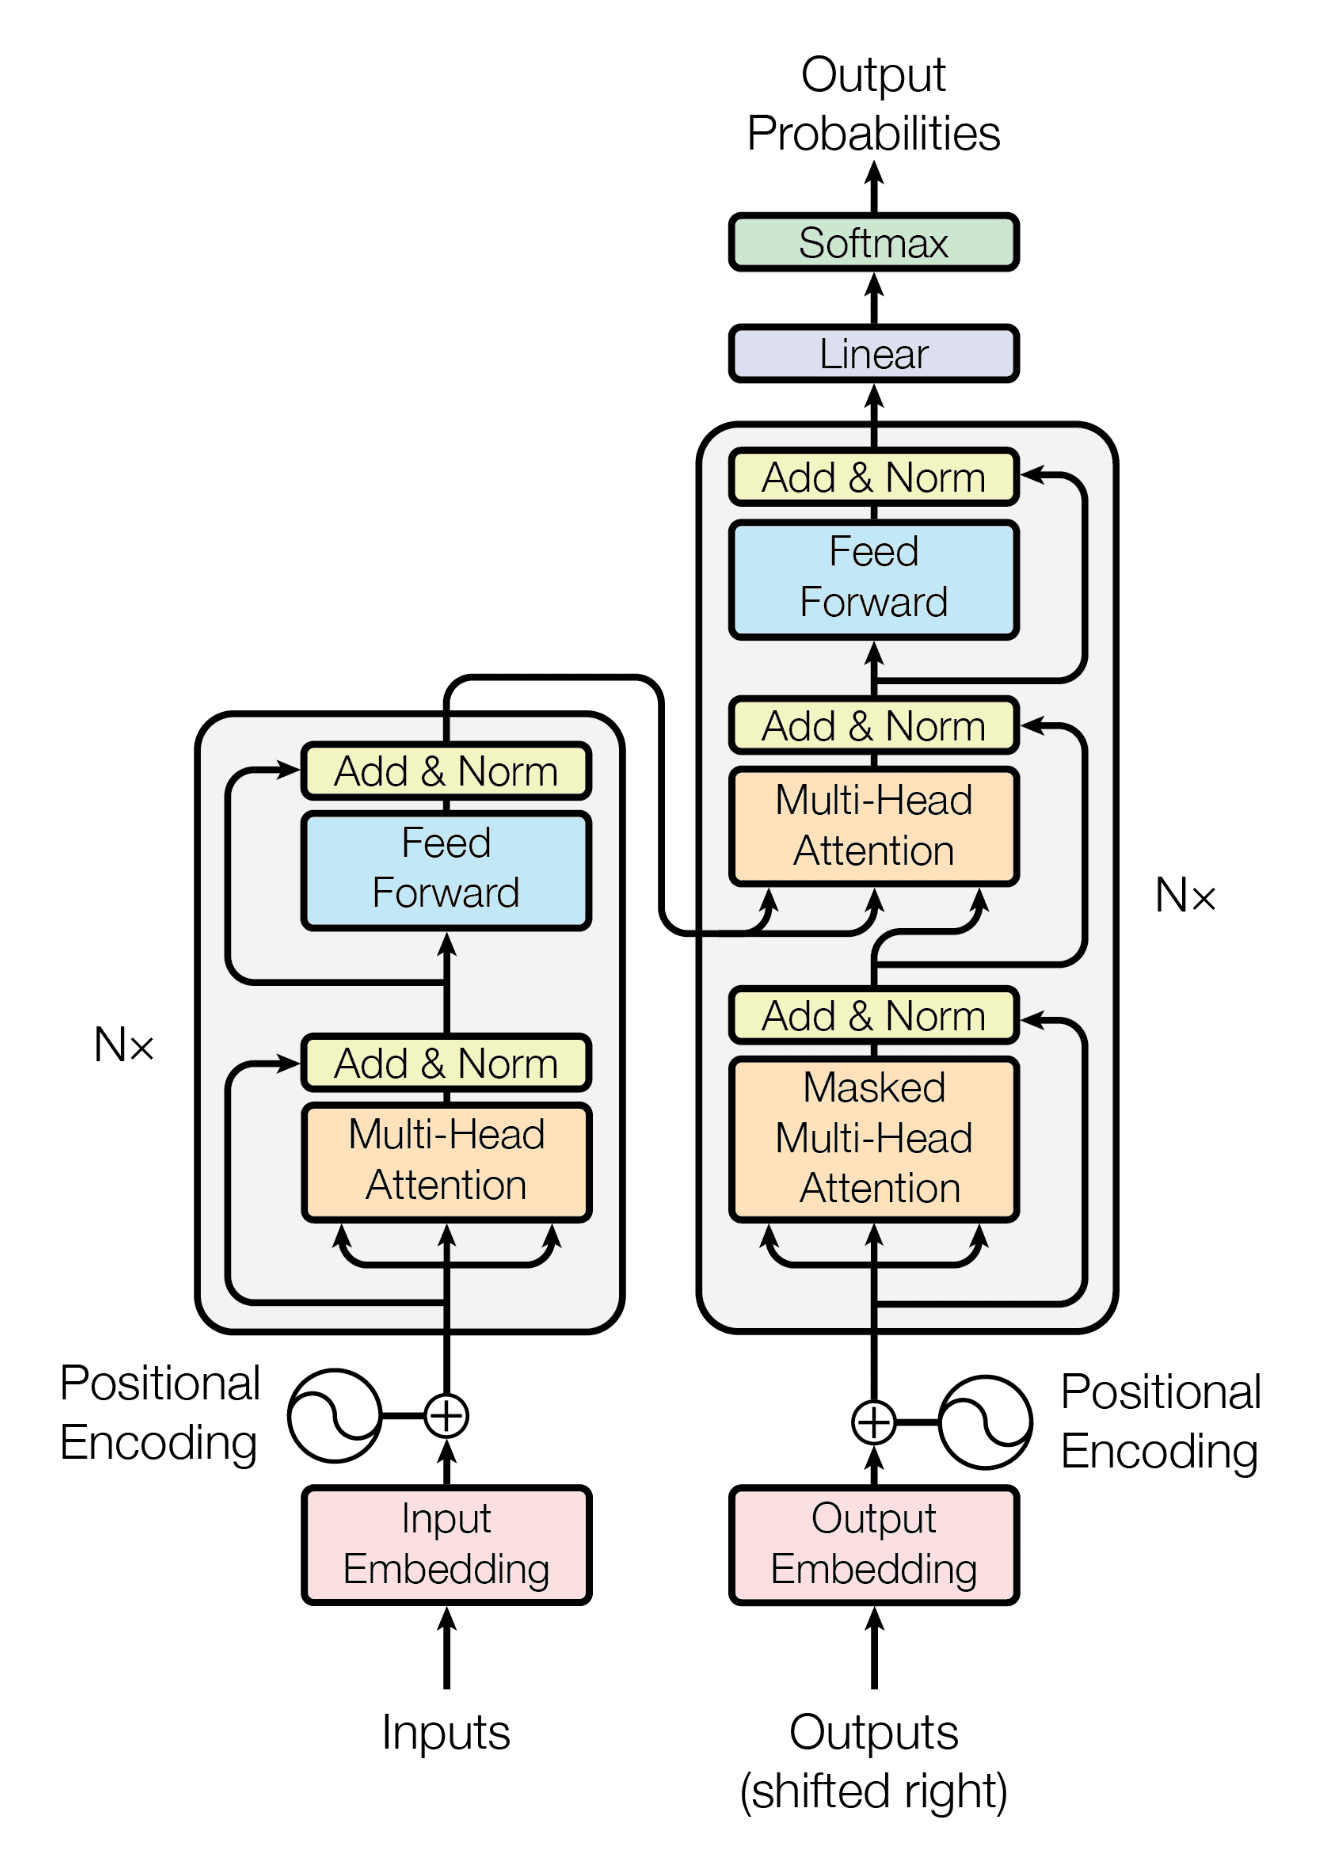
\includegraphics[width=0.7\textwidth]{images/chapter2/transformer.png}
  \caption{\emph{Αρχιτεκτονική Transformer}\\}
  \label{fig:transformer}
\end{figure}
\noindent


Το ζευγάρι \emph{encoder-decoder} εμφανίζεται στη βιβλιογραφία και με τη χρήση αναδρομικών νευρωνικών δικτύων. Ο \emph{encoder} είναι υπεύθυνος για την αντιστοίχηση της διακριτής ακολουθίας συμβόλων εισόδου, $x= [x_1, \cdots, x_n]$, σε μία ακολουθία συνεχών συμβόλων, $z = [z_1, \cdots, z_n]$, ενώ ο \emph{decoder} εφαρμόζει την αντίστροφη διαδικασία για να παράγει την έξοδο, $y = [y_1, \cdots, y_n]$.

\subsection{Επίπεδο προσοχής-Attention}
Προτού τα σύμβολα εισόδου εισέλθουν στο επίπεδο προσοχής, μετατρέπονται σε διανύσματα που ονομάζονται ενσωματώσεις λέξεων\footnote{\url{https://en.wikipedia.org/wiki/Word_embedding}} (\emph{word embeddings}). Στο επίπεδο προσοχής εφαρμόζεται μία συνάρτηση σε κάθε διάνυσμα εισόδου, από την οποία παράγονται τρία νέα διανύσματα για κάθε ένα διάνυσμα $x_i$. Τα τρία διανύσματα αυτά ονομάζονται $query-q$ $key-v$ και $value-v$ και παράγονται από τον πολλαπλασιασμό του διανύσματος $x_i$ με τρεις πίνακες βαρών $W_q$, $W_k$ και $W_v$ αντίστοιχα. Η διαδικασία υπολογισμού του \emph{attention} αποτελεί μία διαδικασία πράξεων πινάκων και εξαιτίας του γεγονότος αυτού πραγματοποιείται πολύ γρήγορα γιατί ο υπολογισμός του μπορεί να γίνει για όλες τις εισόδους $x_i$ ταυτόχρονα.

\subsubsection{\emph{Attention} Σταθμισμένου Εσωτερικού Γινομένου}
Το \emph{attention} σταθμισμένου εσωτερικού γινομένου (\emph{Scaled Dot-Product Attention} υπολογίζεται ως εξής:

\begin{equation}
    \label{eq:attention}
    Attention(Q,K,V) = softmax(\frac{QK^T}{\sqrt{d_k}})V
\end{equation}

όπου στην \autoref{eq:attention}:
\begin{itemize}
    \item $Q$: Πίνακας με τα διανύσματα \emph{query}
    \item $K$: Πίνακας με τα διανύσματα \emph{key}
    \item $d_k$: Η διάσταση των διανυσμάτων \emph{query} και \emph{key}
    \item $V$: Πίνακας μα τα διανύσματα \emph{value}, διάστασης $d_v$
\end{itemize}

\subsection{Attention Πολλαπλής κεφαλής}
Μια παραλλαγή του \emph{scaled dot-product attention} είναι το \emph{attention} πολλαπλής κεφαλής (\emph{multi-head attention}), όπου αντί να εφαρμόζεται μία μονάχα συνάρτηση \emph{attention} εφαρμόζονται πολλαπλές συναρτήσεις με αποτέλεσμα την παραγωγή πολλών διανυσμάτων $q$, $k$, $v$ για κάθε μία από τις εισόδους $x_i$. Αυτή η παραλλαγή βοηθάει ώστε το μοντέλο να μπορεί να επικεντρωθεί σε πολλά τμήματα τις ακολουθίας εισόδου ταυτόχρονα. Η μαθηματική έκφραση του \emph{multi-head attention} φάινεται στην \autoref{eq:multi-head}. Η μάσκα που εφαρμόζεται στο επίπεδο του \emph{decoder} εφαρμόζεται έτσι ώστε οι προβλέψεις για τη θέση $i$ να εξαρτώνται μόνο από τις γνωστές εξόδους που προηγήθηκαν της $i$ και όχι από "μελλοντικές".

\begin{equation} \label{eq:multi-head}
\begin{split}
    MultiHead(Q,K,V) = Concat(head_1, \cdots, head_h)W^O \\
    head_i= Attention(QW_i^Q, KW_i^K,VW_i^V)
\end{split}
\end{equation}

όπου:
\begin{itemize}
    \item $d_{model}$: Η διάσταση των διανυσμάτων εξόδου του μοντέλου
    \item $W^Q \in \mathbb{R}^{d_{model} \times hd_k} $
    \item $W^K \in \mathbb{R}^{d_{model}\times  hd_k} $
    \item $W^V \in \mathbb{R}^{d_{model} \times  hd_v} $
    \item $W^O \in \mathbb{R}^{d_{model}\times  hd_k} $
\end{itemize}

Η έξοδος του επιπέδου \emph{multi-head attention}, αφού πρώτα αθροιστεί και κανονικοποιηθεί, εισέρχεται σε ένα απλό \emph{feed-forward} πλήρως συνδεδεμένο NN το οποίο χρησιμοποιεί συνάρτηση ενεργοποίησης \emph{ReLU}\footnote{\url{https://en.wikipedia.org/wiki/Rectifier_(neural_networks)}}.

\section{Μοντέλο BERT}
Το μοντέλο Αμφίδρομης Αναπαράστασης Κωδικοποιητών από \emph{Transformers} \linebreak(\emph{Bidirectional Encoder Representation from Transformers - BERT}) \cite{bert} αποτελεί ένα προ-εκπαιδευμένο μοντέλο που εστιάζει στην επίλυση προβλημάτων \emph{NLP} και \emph{NLU}. Η αρχιτεκτονική του είναι βασισμένη στα \emph{transformers} και πιο συγκεκριμένα στους \emph{encoders} τους. Στο άρθρο τους \cite{bert} οι \emph{Devlin et al.} παρουσιάζουν δύο παραλλαγές του μοντέλου το $BERT_{BASE}$ και το $BERT_{LARGE}$, με το πρώτο να αποτελείται από 12 \emph{encoders}, 12 \emph{attention heads} και 768 \emph{hidden layers} ενώ το δεύτερο από 24, 16 και 1024 αντίστοιχα.

Για να μπορέσει το \emph{BERT} να χρησιμοποιηθεί σε πληθώρα γλωσσικών προβλημάτων η είσοδος του μπορεί να είναι είτε μία πρόταση είτε ζεύγος προτάσεων, οι οποίες συνδέονται νοηματικά. Η προ-εκπαίδευση του χωρίστηκε σε δύο κατηγορίες προβλημάτων, την συμπλήρωση κενής λέξης (\emph{Masked Language Modeling - MLM}) και την πρόβλεψη επόμενης πρότασης (\emph{Next Sequence Prediction - NSP}). Πιο συγκεκριμένα, τα προβλήματα τύπου \emph{MLM} εστιάζουν στην τυχαία απόκρυψη κάποιον λέξεων της πρότασης εισόδου. Ως πρόβλημα προς επίλυση το μοντέλο πρέπει να προβλέψει τις αντίστοιχες κρυφές λέξεις. Από την άλλη μεριά τα προβλήματα \emph{NSP} εστιάζουν στην πρόβλεψη της επόμενης πρότασης, δεδομένου μιας πρότασης εισόδου. Αυτού του είδους η προ-εκπαίδευση είναι βοηθητική κυρίως σε προβλήματα τα οποία προσπαθούν να προσδιορίσουν την νοηματική σχέση μεταξύ δύο προτάσεων. Παράδειγμα τέτοιων προβλημάτων αποτελούν τα συστήματα \emph{QA}.

Ο τρόπος με τον οποίο το \emph{BERT} μπορεί να χρησιμοποιηθεί σε πληθώρα προβλημάτων είναι η επανεκπαίδευση (\emph{fine-tuning}) του σε κάποιο συγκεκριμένο πρόβλημα. Το \emph{fine-tuning} του μπορεί να επιτευχθεί με την παροχή των κατάλληλων εισόδων και εξόδων στη διαδικασία της επανεκπαίδευσης. Με τον τρόπο αυτό το μοντέλο έχει τη δυνατότητα να επιλύσει προβλήματα QA, κατηγοριοποίησης κειμένου, μετάφρασης και άλλων. Επιπλέον, ακριβώς επειδή έχει αρχικά εκπαιδευτεί σε πιο γενικά αλλά παρόμοια προβλήματα η διαδικασία του \emph{fine-tuning} είναι σχετικά γρήγορη, σε σχέση με το αν γινόταν εκπαίδευση του μοντέλου από το μηδέν.

\section{Μοντέλο Greek-Bert}
Μετά την αρκετά μεγάλη επιρροή του \emph{BERT} στο χώρο της επεξεργασίας φυσικής γλώσσας έγιναν μελέτες του μοντέλου και σε γλώσσες διαφορετικές από τα αγγλικά. Το $2020$, παρουσιάστηκε η αντίστοιχη προσπάθεια για την ελληνική γλώσσα στο άρθρο \emph{GREEK-BERT: The Greeks visiting Sesame Street} \cite{greek-bert} από τους \emph{Koutsikakis et al.} όπου μελετήθηκαν οι αντίστοιχες αρχιτεκτονικές $BERT_{BASED}$ και $BERT_{LARGE}$, με την εκπαίδευση των μοντέλων σε μεγάλο σύνολο δεδομένων της ελληνικής γλώσσας. Η αξιολόγηση των δύο μοντέλων έγινε στα παρακάτω προβλήματα:
\begin{itemize}
    \item Συντακτική Ανάλυση Προτάσεων (\emph{Part of Speech tagging - PoS tagging})
    \item Εξαγωγή οντοτήτων (\emph{Named Entity Recognition - NER})
    \item Εξαγωγή συμπερασμάτων από φυσική γλώσσα (\emph{Natural Language Inference - NLI})
\end{itemize}

Η σύγκριση του έγινε με άλλα μοντέλα τελευταίας τεχνολογίας και η απόδοση του αποδείχθηκε καλύτερη στα \emph{NER} και \emph{NLI}.